\chapter{Einleitung}


\section{Industriepartner}
Variosystems ist ein international tätiges Elektronik- Dienstleistungsunternehmen mit 1100 Mitarbeitern. Es stellt elektronische Baugruppen und Geräte her. In den Produktionsstätten werden PCB mit Bauteilen bestückt und verlötet. \cite{variosystems} 

In dieser Arbeit ist die Variosystems nicht nur der Arbeitgeber, sondern arbeitet auch aktiv mit. In vielen technischen Fragen haben die Ingenieure der Variosystems ihr Know-How eingebracht. Die PCBs für den BeagleBone Black wurden ebenfalls in der Variosystems bestückt.



\section{Motivation}
Die Variosystems bestückt nicht nur fremde PCBs, sie stellen auch eigene Produkte her. Einige dieser Produkte müssen, z. B. für Wartung und Systemüberwachung, mit dem Internet verbunden werden.

Eine mögliche Lösung wäre der BeagleBone Black. Dieser kostengünstige Platinencomputer bringt neben USB und I$^2$C noch diverse andere Schnittstellen, die in der Elektronik üblich sind. Allerdings hat der BBB weder WLAN noch BLE. Ein weiteres Problem ist, dass das Produkt in grösseren Stückzahlen Lieferprobleme hat. Dies ist in der Vergangenheit bereits vorgekommen.

Wenn die Variosystems diesen Platinencomputer selbst herstellen könnte, wäre Sie nicht mehr auf die Lieferbarkeit des BBB angewiesen. Zusätzlich würde die Möglichkeit bestehen, den Computer nach eigenen Wünschen zu modifizieren. So können zusätzliche Funktionen wie BLE und WLAN hinzugefügt werden, und nicht benötigte Funktionen weggelassen werden. Dies spart besonders dann Geld, wenn das Produkt in grossen Stückzahlen hergestellt wird.


\section{BBB}
%TODO BeagleBone Balck als überschrift 
%BBB wurde früher im Text benutz daher dort wo es zu erst benutzt wurde Der BeagleBone Black (kurz BBB) oder Der BeagleBone Black, im weiterm Text als BBB bezeichnet, schreiben

Der BeagleBone Black (kurz BBB) ist, obwohl er nur halb so gross ist wie eine Hand, ein vollständiger Computer. Er wird standardmässig mit einem Ubuntu Linux ausgeliefert. Direkt aus der Packung kann der BBB über ein HDMI Kabel an einen Bildschirm oder Fernseher angeschlossen werden und gestartet werden.
%TODO Er wird standardmässig mit dem auf Linux basierten Betriebssystem Debian ausgeliefert.

Neben einem Micro-HDMI Anschluss hat der BBB auch noch einen Ethernet Port, einen USB Host und einen USB Client Anschluss. Über den USB Client Anschluss kann der BBB an einen anderen PC angeschlossen werden, und so programmiert werden. Der Host Anschluss ist ein normaler USB Prot, der z. B. für eine Maus oder USB Stick verwendet werden kann.
%TODO besser Mini-USB Client
Bei der Entwicklung des BBB wurde auf Massenproduktion und günstige Bauteile optimiert. Dies und die grossen Stückzahlen, die Produziert wurden, führten zu einem sehr günstigen Produkt.

\begin{figure}[!ht]
\centering
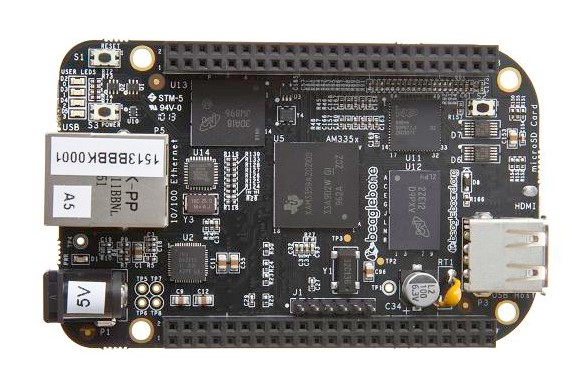
\includegraphics[angle=0,height=5cm]{images/BeagleBoneBlack.jpg}
\caption{BeagleBone Black}
\label{BeagleBoneBlack}
\end{figure}


\section{Aufgabenstellung}
%Auftrag generell
Im Auftrag des Industriepartner Variosystems soll ein eigener, kostengünstiger, auf dem BeagleBone Black basierter Platinencomputer entwickelt werden. Dafür gilt es, ergänzend zu den eigentlichen Funktionen des BeagleBone Blacks, weitere Funktionen wie WLAN, Bluetooth Low-Energy, und GSM/GPRS zu integrieren. Zusätzlich soll ein TFT-Display mit kapazitivem Touch angeschlossen werden, welches von Variosystems gestellt wird. Das ganze soll dann als Einheit aufgebaut werden.

%Herstellbarkeit praktisch
Ziel der Arbeit ist es, dass die Variosystems diesen Computer selber herstellen und nach Wunsch modifizieren kann. Die Produktionspläne sollen so aufbereitet werden, dass die benötigten PCBs bei einem PCB-Hersteller bestellt werden können. Die Bestückung der PCBs erfolgt dann in der Variosystems. Bei den Bauteilen ist ein besonderes Augenmark auf die Lieferbarkeit zu werfen. Damit die Bauteile bestellt werden können, muss eine Bauteilliste, auch "Bill of material" oder kurz BOM, erstellt werden. Diese Liste ist mit der Bestellnummer von üblichen Distributoren wie zum Beispiel Digi-Key oder Mouser ergänzt werden. Standartbauteile, etwa Widerstände, hat Variosystems auf Lager. Bei solchen Bauteilen muss auch die Artikelnummer von Variosystems für das entsprechende Bauteil in der BOM ergänzt werden.

%Modularität, kritischer bereich, 
Die Hardware, und auch die Software, soll möglichst modular aufgebaut sein. Dies bedeutet für die Hardware, dass alle Bauteile für eine bestimmte Funktion, gruppiert und eindeutig erkennbar sein. Ebenso sollen die Bauteile identifiziert werden, welche unbedingt für die Lauffähigkeit des Computers unbedingt benötigt werden. Ein besonderes Augenmerk ist auf die Stellen zu werfen, bei denen die Leiterbahngeometrie relevant ist. Wie etwa bei der Hochgeschwindigkeitsschnittstelle zwischen Prozessor und RAM. Die Softwaretreiber sollen so geschrieben sein, dass die einzelnen Treiber ohne die anderen lauffähig sind. 

%TODO Egemen 
%Software
Zusätzlich zu den Treibern sollten auch Applikationen für die Einzelnen Module entwickelt werden, welche als Demonstration der Funktionen und Beispiele für mögliche Anwendungen verwendet werden sollen.
